\section{Methods*}

The purpose of this chapter is twofold. It will discuss the design and processing decisions that were made for the development of this project, while also giving explanatory insight into how these applied technologies work. I decided that the latter will do more good in this chapter than in the previous one because the theoretical background is directly connected to the choices methods that were applied.

\subsection{Setup*}

The workstation for this study included an Intel i5 processor, 16GB of RAM and most importantly a NVidia Geforce GTX1060/6GB. Neural Networks can be trained more effienctly on GPUs than CPUs. This is because the simpler but highly parallized architecture of graphics chips plays in favour for the needed calculations in deep learning.

The workstation ran Ubuntu 16.04 with the CUDA and cuDNN libraries installed in order to take advantage of the GPU. As the main programming language Python 2 was chosen due to its simple syntax and popularity in the deep learning field. The code of this project is compatible with Python 3 as well. Keras was used as the framework for training models, because its top level syntax allows fast prototyping and testing. The development environment was a Jupyter Notebook, which allowed a flexible execution of code snippets instead of running the entire program for every single change.

The processing of medical image data needed a library that could handle these formats. SimpleITK is a Python binding of the ITK library written in C++. It includes many tools for image processing and is especially popular in the medical field. Other libraries were also used for smaller task. A complete listing can be found on the project's GitHub page, where the entire code is available.

\subsection{Data Analysis*}

The dataset was a collection of three dimensional MR images showing the right human knee. The number of available samples grew during the project. For most of the development time it included 150 images that came from 3 different sources. All images were provided in the MHD file format, which is very common in the medical field. It features lossless compression, as well as certain meta information about each image. The resolution of these samples differed from one source to the other.

\begin{table}[h!]
\centering
\begin{tabular}{l l l r r l}
    Source & Prospective & Perspective & Samples & Maps & Resolution \\
    \hline
    Epi    & Yes         & Coronal     & 80      & 40   & 800x800x41 \\
    Jopp   & No          & Coronal     & 65      & 36   & 512x512x24 \\
    Maas   & No          & Sagittal    & 5       & 0    & multiple \\
\end{tabular}
\caption{Details of available images sorted by their source}
\end{table}

Data provided from Maas et al. featured a sagittal perspective, while all other samples were taken coronal. This mattered because the resolution of all images was roughly 20 times lower on the z-axis. The 65 images from Jopp et al. were another source of retrospective data, of which 36 had segmentation maps. The origin of this data was a previous study that investigated the condition of the epiphyseal plates of Tibia and Femur. A total of 80 MR images were specifically taken for this project. They showed the highest resolution in all dimensions and half of them had segmentation maps.

The total of 76 maps were all manually created by two different people. Each mask featured 3 channels that showed Femur, Tibia and Fibula separately. They did not segment the entirety of each 3D image, but masked a window around the knee cap where the three bones meet.

The candidates chosen for the MRI recording were all german males between the age of 14 and 21. This age was specifically chosen, because it marks the range in which the epiphyseal plates in the knee grow together. Their age appearance was normally distributed with a mean of 17.5 years.

\subsection{Preprocessing*}

The number of parameters in a Neural Network commonly range from hundreds of thousands to hundreds of millions. This complexity allows the model to learn on its own what features of an image are relevant for any given task. It works in conjunction with the fact that high volumes of data are available for the training.

Because of the small dataset that was available for this study, several types of data preprocessing were applied to the images. These techniques do one of three things:

\begin{itemize}
\item Decrease the amount of information per sample
\item Decrease the variance between multiple samples
\item Increase the total number of samples
\end{itemize}

Other preprocessing methods experimented with the difference between 2D and 3D data as well as the influence of separate segmentation channels on the output.

\subsubsection{Cropping, Resizing and Resampling*}

The framing of the raw images included large parts of the thigh and shin to be visible in the picture. Since these weren't relevant for the purpose of the study, they were cropped out. An algorithm was used to detect the center where Tibia and Femur meet and only use a square window around this point.

Although there is no theoretical size limitation to using convolutional neural networks, it is desirable to reduce the spatial resolution to decrease the amount of calculations. 224x224 pixels for width and height still gave enough detail to identify the shape of Femur, Tibia and Fibula.

Resizing the z-axis was problematic, because the resolution was roughly 20 times lower. When scaling along this dimension the segmentation maps of different slices started to blend together and create merged maps of multiple layers. In order to get the images from two different main sources on the same scale, the 41 slices per image of the Epi data were padded with empty pixels to 48 slices. Afterwards every second 2D image was taken to resample to the same 24 slices the data from Jopp et al. showed. It was not possible to do it the other way around and upscale 24 slices to 48, because the interpolated segmentation maps would have been misleading and false.

Throwing away perfectly good data is very uncommon in the machine learning field, especially if datasets are rather small. However, one slice shares a lot of similar information with its neighboring slices and can be seen as a sort of image augmentation between the two. By using the same spatial resolution for both sources the balance between the amount of Epi and Jopp data was kept.

A total of 76 24x224x224 images were now available for training.

\subsubsection{Normalization*}

The normalization of images refers to the process of transforming all samples on the same scale of values. Two techniques for this are popular in the field of deep learning. The first one is called feature scaling, where every sample is normalized between 0 and 1.

\begin{figure}
\[x' = \frac {x - min(x)}{max(x) - min(x)}\]
\end{figure}

The second technique calculates the standard score, where the mean is subtracted from the samples and then divided by the standard deviation.

\begin{figure}
\[x' = \frac {x - \mu}{\sigma}\]
\end{figure}

In this case the mean and standard deviation are not calculated for every image, but for the entire population of training samples. This centers the intensities around the average brightness. When normalizing validation and test sets, it is important to use the mean and standard deviation of the training data, instead of calculating them on their own values.

The standard score presents a more desirable approach, because its mean centering helps to prevent exploding and disappearing gradients in a more effective way. It is also less sensitive to outliers, which frequently appeared in the form of extremely high intensities. 

\subsubsection{N4 Bias Field Correction*}

A bias field is a low frequency nonuniform intensity that is an unwanted byproduct Magnetic Resonance imaging. Several methods have been developed in the past of which N4ITK \cite{Tustison2010} is the de facto standard in the field. This algorithm approximates the nonuniform field and balances intensities using B-Splines. As the name suggests it is included in the Insight Toolkit (ITK) for which SimpleITK delivered an available Python binding. Using the N4 Bias Field Correction with its default settings on a single 24x224x224 image took between 60 and 120 seconds.

\subsubsection{Augmentation*}

Image augmentation is a popular approach to virtually increase the size of the dataset. The general idea is that a neural network will overfit more when learning one sample n times, than learning n alternations of this sample just once. It helps to generalize on new images instead of memorizing patterns in the training data.

Lossless augmentation techniques are those that don't change the values and relative localities in a sample. In 2D these include vertical and horizontal flips, as well diagonal flips, if width and height are equal. Note that any multiples of 90 degree rotations can also be created using a combination of these flips. Although the samples are changed as a whole, they do not vary in respect to their contained values. 

The term "lossless" only refers to the technical change and not necessarily to the semantic change. Flipping a slice of this dataset vertically switches the absolute positions of Femur and Tibia. This might make it harder for the network to distinguish between the two.

Lossy augmentation methods include a variety of image transformations. Common choices include:

\begin{itemize}
\item Horizontal shifts
\item Vertical shifts
\item Rotations
\item Shear mapping
\item Brightness adjustments
\item Contrast adjustments
\item Gamma adjustments
\end{itemize}

For the purpose of this study horizontal flips were implemented to give the impression that images from both knees were available. In addition to this these images were shifted 24 pixels on the horizontal axis to add another type of augmentation. 

Interestingly, these methods did not improve the accuracy of the model. The horizontal flips even hurt the performance and were therefor removed. The horizontal shifts were kept in the training set, so the network would perform better on data that was not perfectly aligned.

\subsubsection{2D and 3D data*}

Although convolutional neural networks are most commonly connected with 2D data such as photos or drawings, they can be applied in any dimensional space. In Natural Language Processing (NLP) 1D convolutions are often used on sentences and in finance they can be applied to time series forecasting. In the medical field where a variety of volumetric data exists, 3D convolutions have become a popular choice for building deep learning solutions.

In the context of neural networks one has to differentiate between volumetric data with one channel and 2D data that consists of multiple color channels. Both are example of 3D data, but the volumetric images features three spatial dimensions, whereas photos feature only two. Convolutions commonly traverse the spatial dimensions, which means photos with multiple channels are usually not subject to 3D convolutions. Instead multiple input channels are fed into a 2D CNN.

Although the dataset consisted of volumetric MRI data, the z-axis showed a 20 times lower resolution than the other two. Not knowing the influence of this situation both 3D and 2D architectures were investigated for this project. The 3D model didn't use any MaxPooling on the already small z-axis. A kernel size of 3x3x3 was used similar to the 3D version of U-Net. The 2D data was created by using each of the 24 slices as a single input image. 

While in theory the spatial information of the z-axis gave the 3D network more contextual information of every slice, the 2D model performed better at the end. The latter was also less computationally expensive and allowed working with data where only single slices where available per sample.

\subsubsection{Separate Bone Maps*}

The initial segmentation maps came with three separate channels for the Femur, Tibia and Fibula. With this information it was possible to train a network that would segment the three bones while still differentiating between them. In theory, this gave the network more context concerning the placement of each bone, but it also was a more complex task to solve. 

In practice, this led to problems with the Fibula, which was not recognized by any of the applied architectures. The channel was always predicted empty. It's appearance in the images accounted for 3.4\% of the segmented area, whereas the Tibia made up 41\% and the Femur accounted for the remaining 55.6\%. This led the network to learn that an empty prediction of this channel is effective in 96.6\% of the cases, which is very accurate on its own. Instead of spending capacity on improving a channel that only makes up a tiny fraction of the end result, the network improved the performance of Femur and Tibia.

The only successful method was training a separate model for each of the three bones. Every empty ground truth segmentation resulted in the highest possible score, which meant the model learned first to make only empty predictions. The only way to improve from here was to find the Fibula in the non-empty slices and segment its region. This was different from the tests before, where the unsatisfactory performance of the Fibula was balanced by making more accurate segmentations from the other two bones.

For another experiment the three channels were merged to create a network that would segment any type of bone in the image. Not only did this solve the problem with the Fibula as well, but the predictions of Femur and Tibia were also more accurate. The network didn't need to learn anymore that the global position in the image accounts for whether or not an object should be segmented. Instead it could segment any kind of bone in any position in the image. It was decided to continue with this approach for further tests, but the same architecture can be used on single bone channels as well. 

\subsubsection{Training, Validation and Testing Sets*}

The data was split into three subsets of which each was used for a different purpose. The training set is commonly the largest of the three and contains the data that is applied to the actual learning process. It's the only portion of the data the network will draw direct conclusions from. 

The validation data is used to regularly measure the performance of the model and check whether overfitting occurs or not. If the accuracy of the validation set drops below the results of the training data, the network is starting to memorize the data it knows rather than generalizing on the concept. 

The third subset is referred to as the testing data. In contrast to the validation set it's only used once in the very end, to give a final score. The idea is that by building a model based on the validation results a certain amount of information bleed occurs, where the network will implicitly learn from the validation data. To prevent biased end results the testing data is used as a last performance reference.

\subsection{Architecture*}

The architecture of most classification CNNs use a recurrent combination of convolutional and pooling layers. By combining the local learning patterns of convolutions with the spatial reductions of pooling, the input is compressed to a dense representation of its most important features.

As mentioned in 3.2.5 a segmentation can be seen as a classification for every pixel. As such early CNN segmentation models used small patches of the input image to only predict a single pixel through a classification pipeline. Afterwards a full segmentation map was assembled using each of these pixels. This process was very slow and it also prevented the network to have a field of view larger than the inserted patch.

An improvement for segmentations came through architectures referred to as encoder-decoder models. The encoding process describes the same spatial compression used in classification networks. Afterwards in the decoding step the spatial resolution is brought back to its original shape and further processed by additional convolutions. This yields huge speed improvements, while also increasing the accuracy of the prediction. Encoder-decoder networks are the de facto standard in the current field of image segmentation and were the initial starting point for building an architecture.

\begin{figure}
\centering
\par
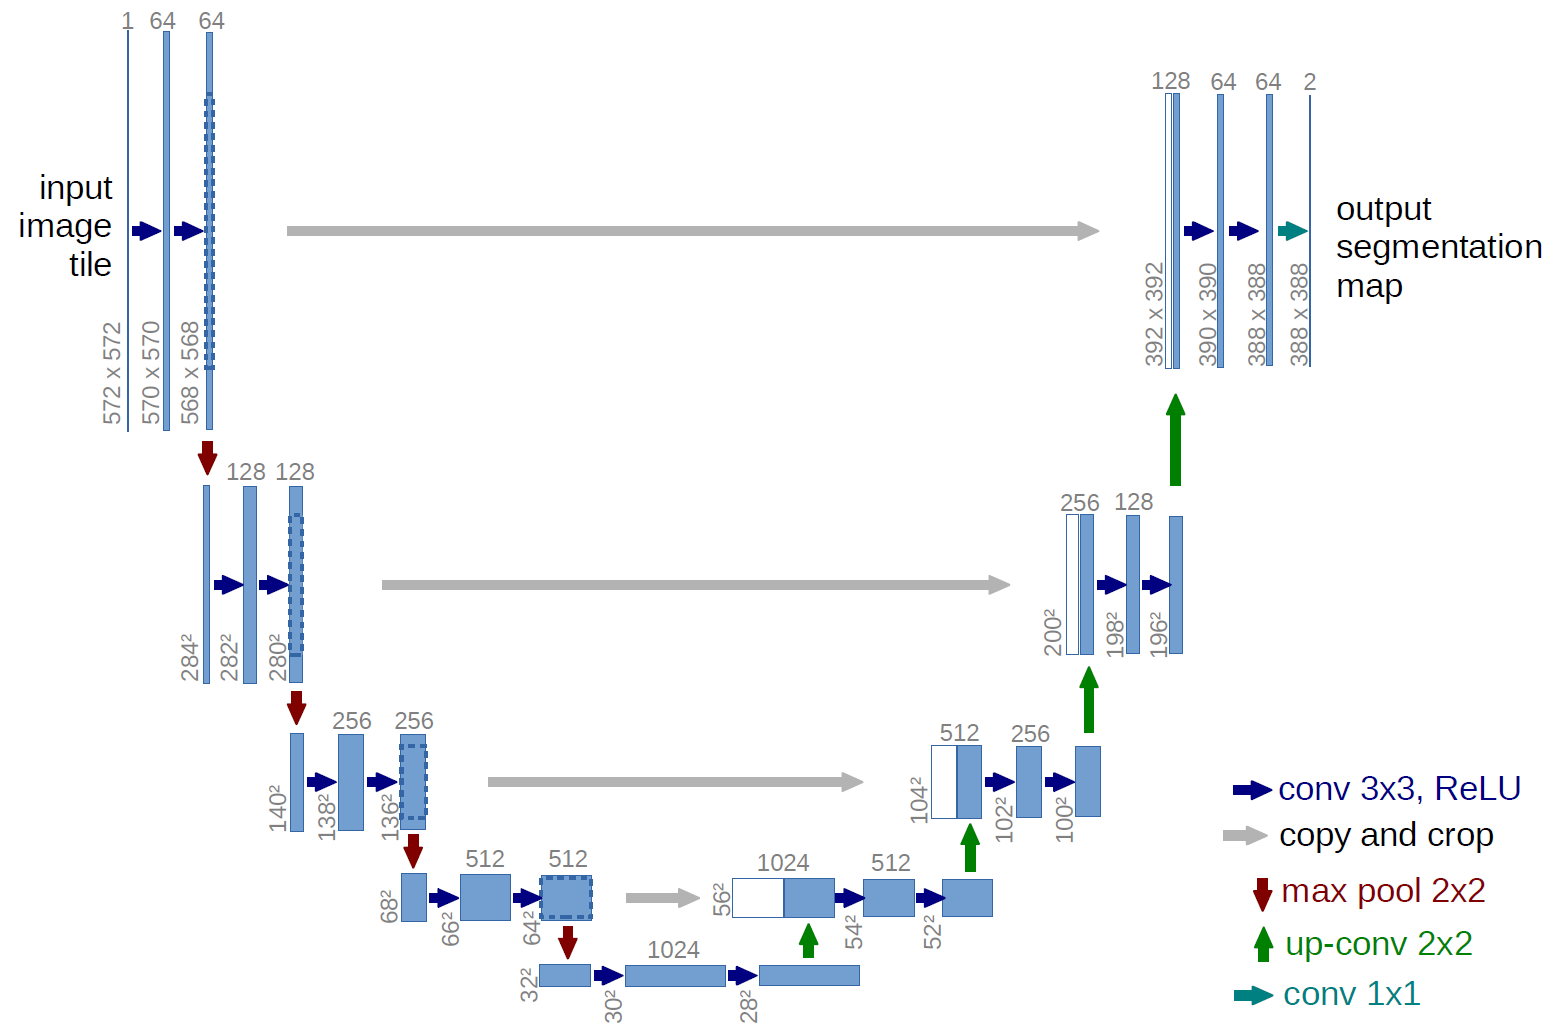
\includegraphics[width=1.0\textwidth]{imgs/unet.png}
\caption{Visualization of the U-Net architecture}
\par
\end{figure}

Figure 3 shows a specific implementation of an encoder-decoder model known as U-Net \cite{Ronneberger2015a}. It has been successfully used on a variety of projects in and outside the medical field. The contracting side on the left shows a similar architecture to classification CNNs, after which the process is mirrored on the expanding side.

The following subchapters will discuss key elements that go into the design process of such an architecture. It was also analyzed how technologies that were introduced after the U-Net paper could possibly improve the performance on this dataset.

\subsubsection{Channels, Growth Rate and Depth*}

The number of parameters in a neural network has a strong correlation with its learning capacity. By adding more nodes that can be adjusted during training, the model can approximate a more complex function that transforms the input into the output. The downside is that a larger parameter count will also increase the possibility of overfitting the data. A convention in the field of CNNs is to gradually increase the number of channels, while the spatial resolution is reduced due to the use of MaxPooling. U-Net also shows this behavior on the left side of its architecture.

A test was set up that compared the original U-Net against 5 smaller variants. They varied in the total number of paramaters and how the number of channels changed from one layer to the next.

\begin{table}[h!]
    \centering
    \begin{tabular}{| l || r | r | r | r | r | r | r | r | r || r |}
    \hline
            & C1   & C2   & C3   & C4   & C5   & C6   & C7   & C8   & C9  & Param. \\ 
    \hline
    Model A &   32 &   32 &   32 &   32 &   32 &   32 &   32 &   32 &  32 & 211k      \\
    \hline
    Model B &   16 &   24 &   36 &   54 &   81 &   54 &   36 &   24 &  16 & 340k      \\
    \hline
    Model C &   48 &   48 &   48 &   48 &   48 &   48 &   48 &   48 &  48 & 474k      \\
    \hline
    Model D &    8 &   16 &   32 &   64 &  128 &   64 &   32 &   16 &   8 & 485k      \\
    \hline
    Model E &   32 &   48 &   72 &  108 &  159 &  108 &   72 &   48 &  32 & 1,358k      \\
    \hline
    U-Net   &   64 &  128 &  256 &  512 & 1024 &  512 &  256 &  128 &  64 & 31,000k      \\
    \hline
    \end{tabular}
    \caption{Convolution blocks 1 to 9 of the candidates with their respective output channels and total number of parameters}
\end{table}

Training U-Net was very slow in two regards. Each training step lasted 6 times longer compared to the smallest model, while it also took 25 times more training steps to reach the same results. Since it was also overfitting to a large amount, it was not trained until the end. The second largest model E also overfitted on the training data and never achieved comparable results to the other 4 models.

D started with 8 channels which were than increased by a factor of 2, whereas B started out larger but only increased the channels by a rate of 1.5. Although it being the smaller model B showed a higher accuracy in the end. It was concluded that the initial number of output channels has a larger effect on the result than the growth rate.

This theory was supported by the results from A and C, both of which kept their initial number of channels throughout the network. These two showed the highest scores in comparison to the other models, while keeping their size relatively small. Since their results were identical model A was kept because of its faster training speed. It was interesting to see that the smallest model performed best across the candidates.

The original U-Net featured a depth of 5 convolutional blocks until reaching the bottom of the "U"-shape. It was also investigated that a depth of 6 would not improve performance, while a depth of 4 decreased the accuracy. Model A was therefor left unchanged.

\subsubsection{Skip Connections*}

U-Net uses skip connections to copy values from the left side to the corresponding layer on the right side. This improves performance because otherwise spatial information would get lost while contracting the input. An experiment showed that removing these paths indeed hurt the performance badly.

ResNet \cite{He2015a} is another popular classification architecture that was the first to use residual connections. These are another type of skip connection that bridge the beginning and end of a convolutional block. They are also one of the main reasons CNNs can be expanded to depths of thousands of layers. Since their use in the industry has found great success in many models, they were also applied in this network. However they did not have an impact on the performance or the training speed, which is why they were removed.

\subsubsection{Dropout*}

Dropout is a popular regularization technique that randomly zeros out a fraction of the nodes during training \cite{Srivastava2014}. It is understood that this helps the model to generalize better and reduce overfitting on a given dataset. Well known image classification architectures like VGG16 \cite{Simonyan2014a}, SqueezeNet \cite{Iandola2016a} or AlexNet \cite{Krizhevsky} use Dropout near the end of the network. Similarly U-Net uses Dropout at the end of the contracting path to prevent overfitting.

Since a single unit of dropout with a rate of 0.5 is common in other architectures, this was also chosen as a first option. Other tests included adding multiple dropout units between the convolutions on the contracting side, which led to slower training and lower scores. Adding dropout on the expanding side is rather unusual and also didn't perform well in the tests. In the end the initial candidate was chosen for future trainings.

\subsubsection{Activation Functions*}

Activation functions sit between layers in a network to introduce a non-linearity. Otherwise the dense and convolutional operations could be regenerated to a simple linear transformation and remove the benefits of building a deep model.

\begin{figure}[H]
\[
f(x) =
\begin{cases} 
0 & \text{if } x < 0  \\
x & \text{if } x \geq 0
\end{cases}
\]
\caption{Rectified Linear Unit (ReLU)}
\end{figure}

The rectified linear unit or ReLU \cite{Nair} is the default recommendation for an activation function in modern neural networks. It's defined as the maximum of 0 and the input value, and can be described as a non-linear function made up of two linear pieces. Because of this it preserves many of the properties that make models easy to optimize and generalize well on new data \cite{Goodfellow2016}.

Since the introduction of ReLU other variants have built on its success like PReLU \cite{He2015}, LReLU and ELU \cite{Clevert2015}. The latter titled exponential linear unit shows the same linear behavior for positive inputs, but adds an exponential function to negative values instead of erasing its value.  This has showed further improvements by keeping the mean of values centered at 0 while only being slightly more computationally expensive.

\begin{figure}[H]
\[
f(x) =
\begin{cases} 
e^x - 1 & \text{if } x < 0  \\
x & \text{if } x \geq 0
\end{cases}
\]
\caption{Exponential Linear Unit (ELU)}
\end{figure}

ELU showed superior results in comparison to ReLU and was chosen for all future tests.

\subsection{Training*}

The training is where the actual learning takes place and its process is inspired by how humans improve their performance on tasks. When opposed with a difficult question the first step would be a simple guess of what the answer might be. In a second step this information is compared to the right answer and processed by the brain accordingly.

Similarly, training of a neural network consists of two parts. In the first step the input is fed forward through the network and an answer prediction is made. In the very beginning this is just a random guess, because ANNs are initialized with random values. The prediction is then compared to the ground truth and a performance measure is calculated. This metric can be fed backwards through the network in order to optimize the parameters in the model. These two steps are called forward and backward propagation.

\subsubsection{Metrics and Loss Functions*}

Metrics are used in deep learning to measure the performance of a model. For example the accuracy is often chosen to describe how well a neural network is doing on a classification task. An accuracy of 0.9 indicates that 9 out of 10 samples are classified correctly.

\begin{equation}
Accuracy = \frac{TP+TN}{TP+TN+FP+FN}
\end{equation}

In the formula above T and F indicate whether a prediction was true or false. P and N stand for a positive or negative outcome.

The result of a loss function is a metric that will be minimized during the backpropagation process. In order to be used with gradient descent it needs to be differentiable. That is why the accuracy cannot be used as a loss function. It is a binary metric that works with true or false values and not with probabilities.

In situations like these a surrogate function is used that has a high correlation with the target metric. For classification problems this is often the cross entropy. Because a segmentation can be seen as a classification for every output pixel, it was also chosen as a candidate for this study.

\begin{equation}
Cross Entropy = Insert here
\end{equation}

Another option was the F1 score, which is a specific implementation of the F-Measure when beta is 1. 

\begin{equation}
F_\beta score= \frac{(1 + \beta^2) TP}{(1+\beta^2)TP+\beta^2FN+FP}
\end{equation}

Although the F1 score is commonly applied as a binary measure and therefore not differentiable, a "soft" version can be used that accounts for continuous probabilities. To use it as a loss function where 0 describes the best possible outcome the F1 loss was defined as 1 - F1 score.

\begin{equation}
F_\beta loss = 1 - F_\beta score
\end{equation}

The value of beta can be adjusted to change the emphasize between precision and recall. Precision describes how much of the predicted area was true, whereas recall describes how much of the ground truth was recognized by the model. This can be useful for datasets with high imbalances between classes, like this study showed between Fibula, Femur and Tibia. 

Therefor the F2 score was tried for the three channel segmentation, where the Fibula could not be recognized. Although this model showed better scores regarding recall the Fibula was still not segmented.

\begin{equation}
Precision = \frac{TP}{TP+FP}
\end{equation}

\begin{equation}
Recall = \frac{TP}{TP+FN}
\end{equation}

To test whether the F1 loss or the cross entropy showed better results, both loss functions were used in separate runs to compare their segmentations. The F1 trained model showed better results regarding the F1 score and the cross entropy model showed better results on the cross entropy loss. In regards to Precision, Recall, Accuracy and Intersection-over-Union (IoU) the performance of F1 trained network showed higher scores.

Another test run used both loss function at the same time. This was done by feeding the output of the second to last layer into two separate segmentation outputs. Each of these last layers were trained with the F1 loss and cross entropy loss respectively. All previous layers were therefore trained by the sum of both loss functions. This architecture matched the best results of the previous runs in a single model, but also increased the training time by 30\%.

Evaluating these two outputs on the other metrics played in favor for the F1 loss output. Combining both maps didn't improve the scores any further. Since the cross entropy was chosen as a surrogate function and not as a performance metric, all future tests used only the F1 loss. This delivered faster training than the dual output method.

\subsubsection{Optimizer*}

The previous chapter provided an overview of the loss function, which measures the performance of a prediction during the training process. This chapter discusses how the result can be used to execute the actual optimization step.

The derivative of a single variable function defines the slope of this function at any given point. Knowing this, one can tell in which direction the original function declines. Adjusting the independent variable along the descent of a loss function will minimize the error in respect to its dependent variable.

The gradient is the derivative for functions of multi-dimensional inputs, such as the loss functions used in deep learning \cite{Chollet2017}. A process that minimizes its result is called gradient descent. While it is possible to determine its minimum analytically, it is intractable for artificial neural networks due to the high number of parameters.

Instead the stochastic gradient descent (SGD) is used which will use a random batch of the training data and iteratively adjust the parameters in small steps. SGD is the basis for all common ANNs, but over the years different variants were introduced to the field.

The Adam optimizer is such a variant, which enhances SGD amongst other things by using what's called an "adaptive momentum estimation". This is also where its name derives from. It adaptively adjusts the learning rate which defines how much the parameters will be changed in one training step. By incorporating the previous and current shape of the slope Adam can tremendously speed up the training.

\subsubsection{Batch Size*}

The number of random samples per training step is referred to as the batch size. In the past it was believed that larger batches led to something called the generalization gap \cite{Keskar2016}, where the accuracy of a model would drop if it was trained on particularly large batches. Recent work by Hoffer at al. \cite{Hoffer2017} suggests other reasons for this drop in accuracy. While common batch sizes range from 32 to 256, Goyal et al. showed accurate results using 8192 images per batch when training a model on ImageNet \cite{Goyal2017}.

Using batches smaller than 32 samples can introduce a different kind of problem. Having too few data points that don't represent the mean of the data well, may lead to slow and unstable training.

Based on hardware limitations the largest possible batch sizes ranged from 24 to 48 samples depending on the current architecture. Whatever could be fit into memory was used for these experiments. Exceptions occurred when working with 3D convolutions in which case the batch size was limited to 4 samples.

\subsubsection{Learning Rate Policy*}

One full iteration over the training samples is referred to as an epoch and the learning rate policy describes how the learning rate is changed from one epoch to another. With the introduction of adaptive optimizers like Adam or RMSProp there has been a lower emphasize on this topic. Learning rates that were set too high or too low, will be adjusted by the optimizer after a few iterations. Even though this reduces the number of possible defects, a lot of training time can be saved with the right policy.

10 epochs were run at different learning rates to compare initial results and to examine the point at which the model wouldn't converge at all. 0.002 was the highest rate at which the model started training, but 0.001 resulted in the best score.

\begin{figure}[H]
\[
lr(x) = \frac{1}{1 + decay * x}
\]
\caption{Learning rate at epoch x based on the decay value}
\end{figure}

After the model stopped to improve at epoch 65 the learning rate was changed to 0.0001. This gave a small boost of accuracy. In order to have a smooth transition between learning rates, the decay was set to 0.001. This meant that the initial learning rate of 0.001 would reach 0.0001 after 68 epochs and then continue to decrease even further.

\subsubsection{Early Stopping*}

Neural networks will continuously minimise the loss on the training set. This result needs to be validated on data the network hasn't seen before. At a certain point during training the performance on the validation set will start to decrease, because the model is overfitting on the training data. The number of iterations to reach this point is dependent on many hyperparameters, as well as the random values the network has been initialized with. As such it's difficult to calculate how many epochs the training will need to reach its peak.

Early stopping is a simple technique that will end the training process as soon as the model stops improving on the validation data. In order to do this, a patience is defined how long the network should continue training after the score has stopped increasing. This is important because not every epoch will lead to a new best score on the validation data.

For test runs in this study a patience of 9 was selected, which meant the training would stop after 10 epochs without improvement. Depending on the architecture and other hyperparameters this point was reached after 30 to 60 epochs. For the last training with the final set of hyperparameters the patience was increased to 19, which didn't improve the accuracy.  This was also a verification that the initial value of 9 was a good fit for this problem.

\newpage
